\chapter{Quantum machine learning}

\section{Data encoding}

\section{Quantum neural networks}

\subsection{QNN versus NN}
Fisher's iris dataset is perhaps the most used dataset for classification in statistics, containing samples of three different species of iris flowers. For each species, there are 50 samples, each with four features: sepal length, sepal width, petal length, and petal width. Like in \cite{abbas2021}, only the two first species are considered, which happen to be linearly separable in the feature space.

To compare the performance of the QNN and the NN, architectures suited for binary classification parametrised by exactly 8 parameters are used. The QNN structure is shown in \cref{fig:qnn_vs_nn_models}. The four dimensional input data $\bm{x}$ is mapped to some quantum state $\ket{\psi{\bm{x}}}$ using the ZZFeatureMap with two repetitions, which is a second-order Pauli-Z evolution circuit. This feature map is essentially a mix of rotation around the Z axis parametrised by the input features or functions thereof and CNOT and Hadamard gates. The quantum state is then evolved by a the RealAmplitudes ansatz. All four qubits a rotated in the Y direction by some parameter before CNOT-gates are applied pairwise, for a final parametrised rotation in the Y direction, for a total of 8 parameters. For details on the components, see Qiskit's documentation \cite{qiskit} or the original paper \cite{abbas2021}. The parity of the output 4-bit string is interpreted as the prediction, and with 100 shots used, the model gave a probability for each of the two iris classes. Both exact simulations and noisy simulations were performed, with the latter using noise modelled after the 27-qubit IBM Montreal architecture, the actual hardware used in the original paper.

\begin{figure}
    \centering
    \begin{quantikz}
        \lstick[wires=4]{$\ket{0}^{\otimes 4}$} & \gate[wires=4]{\text{ZZFeatureMap}(\bm{x})} & \gate[wires=4]{\text{RealAmplitudes}(\bm{\theta})} & \meter{} \\
        & & & \meter{} \\
        & & & \meter{} \\
        & & & \meter{} \\
    \end{quantikz}
    \caption{Structure of the QNN used for classification of the iris dataset. The first block maps the input data $\bm{x}$ to the quantum state $\ket{\psi(\bm{x})}$, before the second block is the variational circuit, parametrised by $\bm{\theta}$. Finally, all qubits are measured, where the parity is interpreted as the prediction.}
    \label{fig:qnn_vs_nn_models}
\end{figure}

The classical neural network was a standard feed-forward model, with a 4-1-1-1-2 layered structure without biases, giving a total of 8 parameters. The activation functions were leaky ReLUs,
\begin{equation}
    \text{LeakyReLU}(x) = \begin{cases}
        x     & x \geq 0 \\
        0.01x & x < 0
    \end{cases},
\end{equation}
and the output layer used a softmax activation function.

Both models were implemented using PyTorch, with the QNN being implemented using Qiskit's PyTorch interface. Consequently, the models could be trained in the exact same manner, using the Adam optimiser with a learning rate of 001. The models were trained for 100 epochs, with the loss function being cross-entropy.

For validation, 10-fold cross-validation was used. That is, the dataset was split into 10 equal parts or \textit{folds}. Each fold us used as the validation set once, their accuracies being recorded during the training with the other nine folds. The mean accuracy over the 10 folds was used for the final performance metric, shown in \cref{fig:iris_training}.

As in the original paper, the QNN converges much quicker and more consistently, with an out-of-fold accuracy of 100\% for all ten folds. The NN, on the other hand, requires more iterations to converge and does not always do so. In some cases, the model diverges and only predicts one class, which is why the out-of-fold accuracy is not 100\% for all folds.


\begin{figure}
    \centering
    \begin{tikzpicture}
        \begin{axis}[
                width=0.8\textwidth,
                xlabel={Iteration},
                ylabel={Out of fold accuracy},
                grid = major,
                legend pos=south east,
                legend cell align={left},
                % add 1 to x axis
            ]
            \addplot[mark=none, color=blue] table[x expr=\coordindex+1, y index=3, col sep=comma] {../code/iris/results/mean.csv};
            \addplot[mark=none, color=red] table[x expr=\coordindex+1, y index=2, col sep=comma] {../code/iris/results/mean.csv};
            \addplot[mark=none, color=green] table[x expr=\coordindex+1, y index=1, col sep=comma] {../code/iris/results/mean.csv};
            \legend{
                Noisy QNN,
                Exact QNN,
                Classical NN
            }
        \end{axis}
    \end{tikzpicture}
    \caption{Mean accuracy during training for the iris dataset using 10-fold cross validation. All models have 8 parameters and are trained using the Adam optimiser with a learning rate of 0.1, using cross-entropy as the loss function. Due to the computational cost, the noisy (simulated IBM Montreal backend) QNN was only trained for 10 epochs due to the computational cost.}
    \label{fig:iris_training}
\end{figure}

\subsection{Quantum convolutional neural networks}
Testing a QCNN on synthetic data shown in \cref{fig:qcnn_data}; classify pictures as either horizontal or vertical lines. The model without errors achieve 100\% accuracy on both training and test data, while the noisy model only managed around 90\% accuracy on the training data and 80\% on test data. The loss function of the noisy and exact model during training is shown in \cref{fig:qcnn_loss}.


\begin{figure}
    \centering
    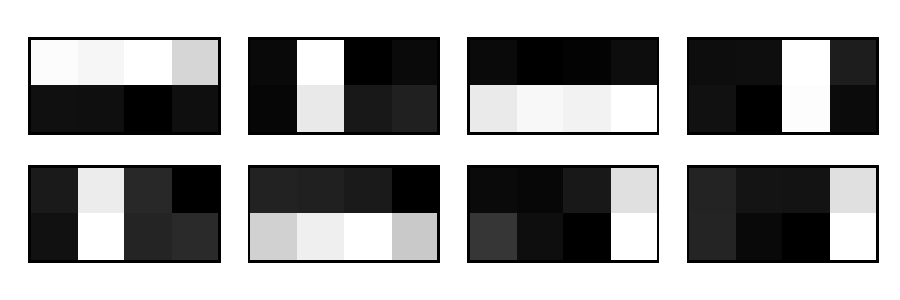
\includegraphics[width=0.8\textwidth]{../code/qcnn/data.pdf}
    \caption{Synthetic data for the QCNN.}
    \label{fig:qcnn_data}
\end{figure}


\begin{figure}
    \centering
    \begin{tikzpicture}
        \begin{axis}[
                width=0.8\textwidth,
                xlabel={Iteration},
                ylabel={Loss},
                % legend pos=north west,
                % legend style={at={(0.5,1.03)},anchor=north},
                grid=major,
            ]
            \addplot[mark=none, color=blue, width=] table[x index=0, y index=1, col sep=comma] {../code/qcnn/optim.csv};
            \addplot[mark=none, color=red] table[x index=0, y index=2, col sep=comma] {../code/qcnn/optim.csv};
            \legend{Noisy QCNN, Exact QCNN}
        \end{axis}
    \end{tikzpicture}
    \caption{Loss function of QCNN model during training with both exact simulations and noisy.}
    \label{fig:qcnn_loss}
\end{figure}


